\newpage

\section*{ $^{164}$Dy(n,$\gamma$)$^{165}$Dy }

Power Level: 100 kW(th) \\
Time at Power: 60.0 s \\
Wait Time:  2.0 h \\
Counting Time:  2.0 m \\
Total Activity at Removal: 1.39e+03 $\mu Ci$

\begin{table*}[h]
\centering
\begin{tabular}{ |c|c|c|c|c|c| }
 \hline
 Position & Mass $mg$ & Counting Activity $\mu Ci$ & Area (Counts) & Error \% \\
 \hline 
 1 & 1.29 & 1.62e+02 & 2.06e+06 & 0.0697 \\ 
\hline
 2 & 1.29 & 2.46e+02 & 3.13e+06 & 0.0566 \\ 
\hline
 3 & 1.29 & 2.27e+02 & 2.88e+06 & 0.0589 \\ 
\hline
 4 & 1.29 & 1.33e+02 & 1.68e+06 & 0.0771 \\ 
\hline
\end{tabular}
\end{table*}

\begin{figure}[h]
\centering
\begin{subfigure}{.5\textwidth}
  \centering
     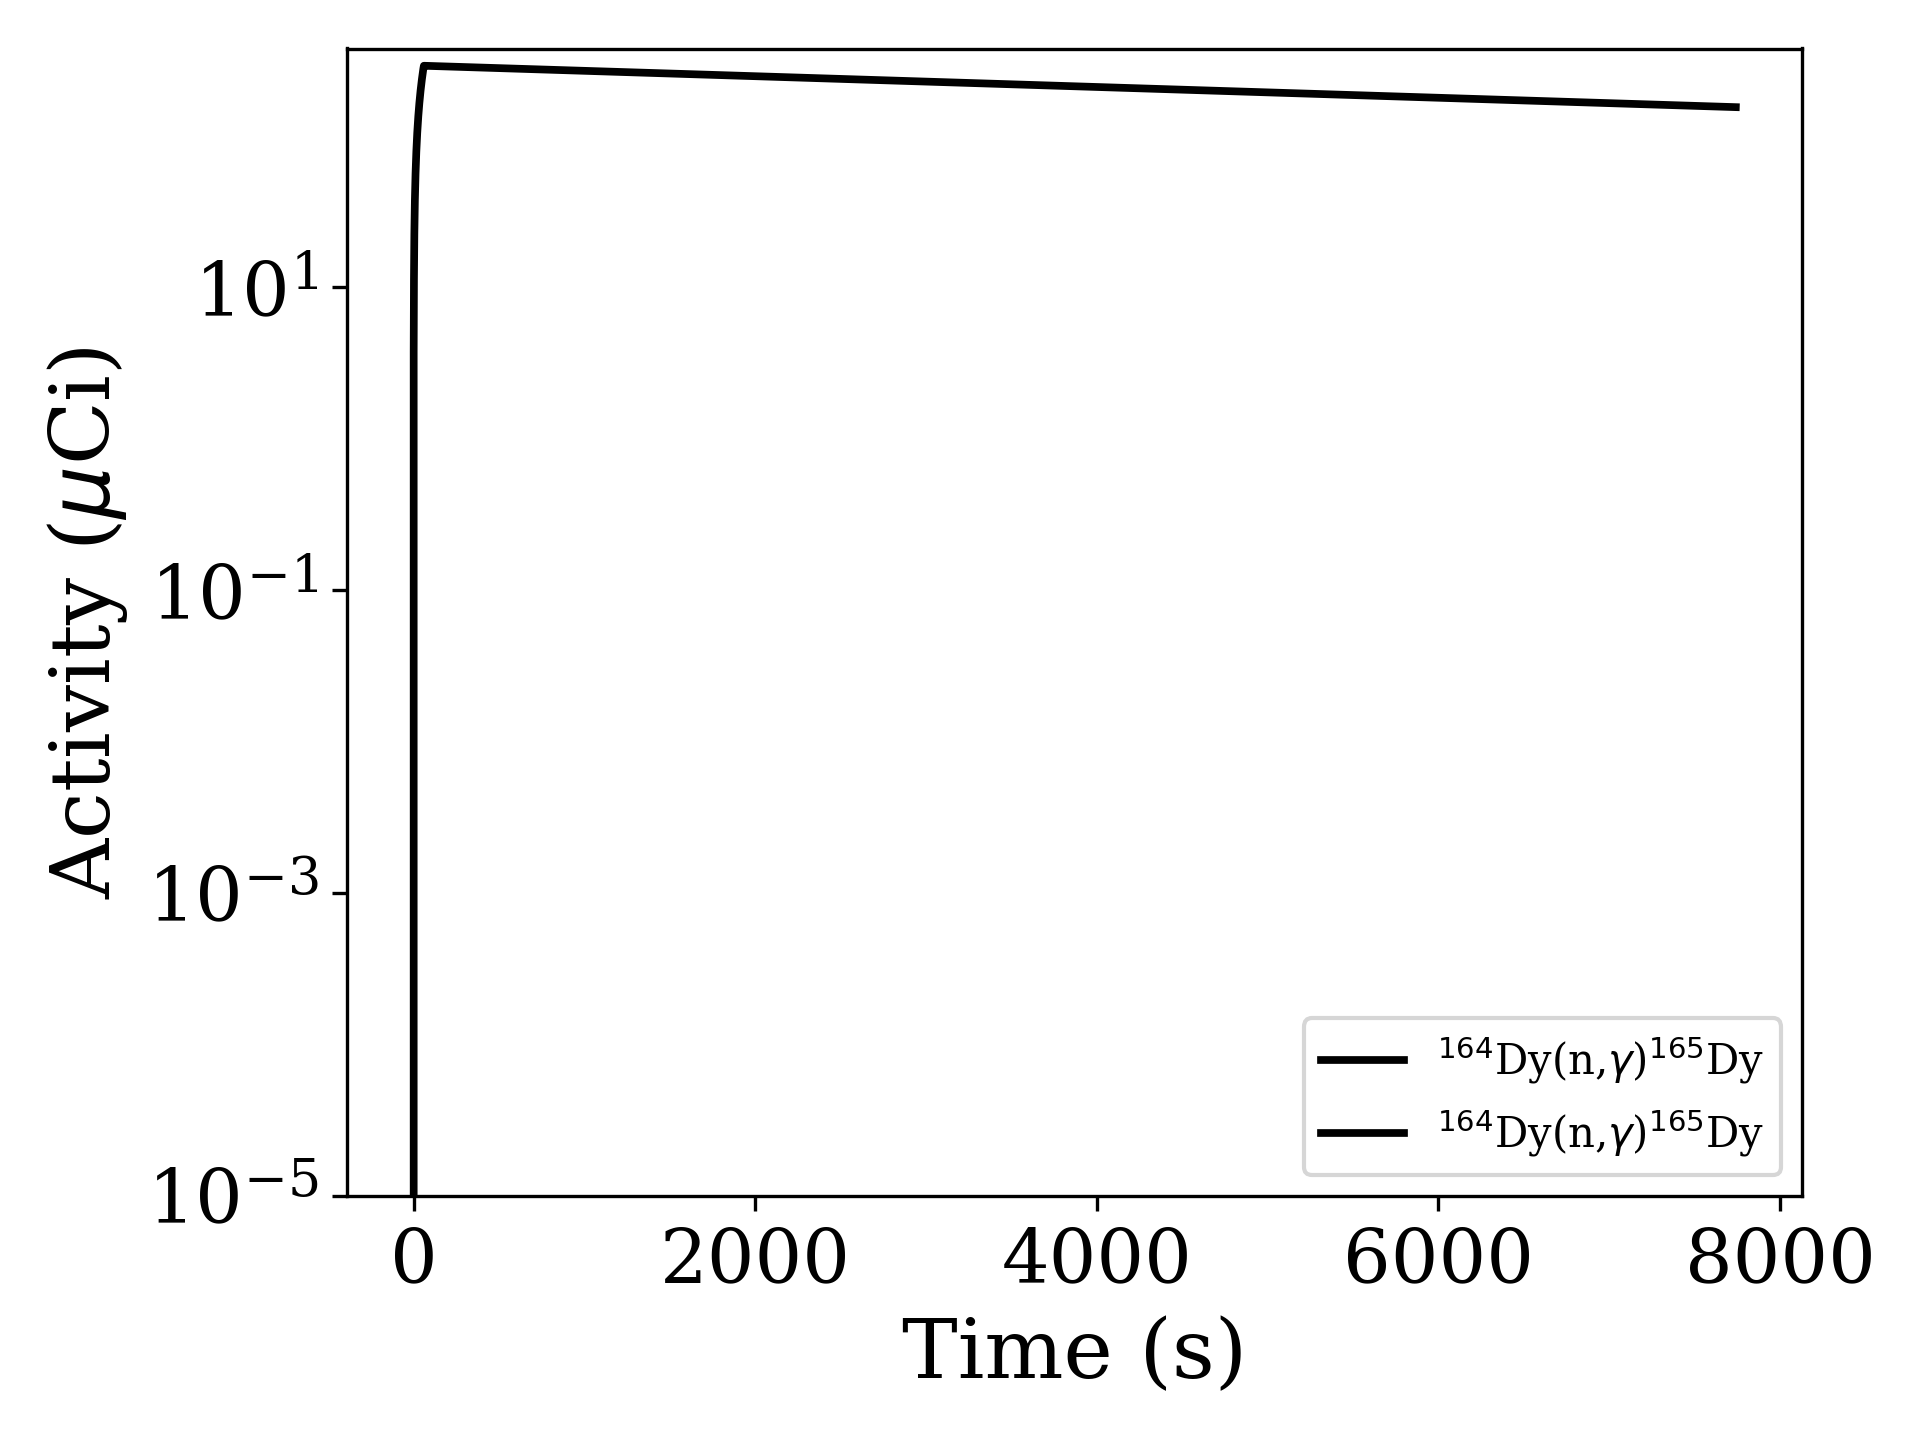
\includegraphics[width=.8\textwidth]{plot/Dy-164(n,gamma)Dy-165_library1} 

  \caption{A subfigure}
  \label{fig:sub1}
\end{subfigure}%
\begin{subfigure}{.5\textwidth}
  \centering
     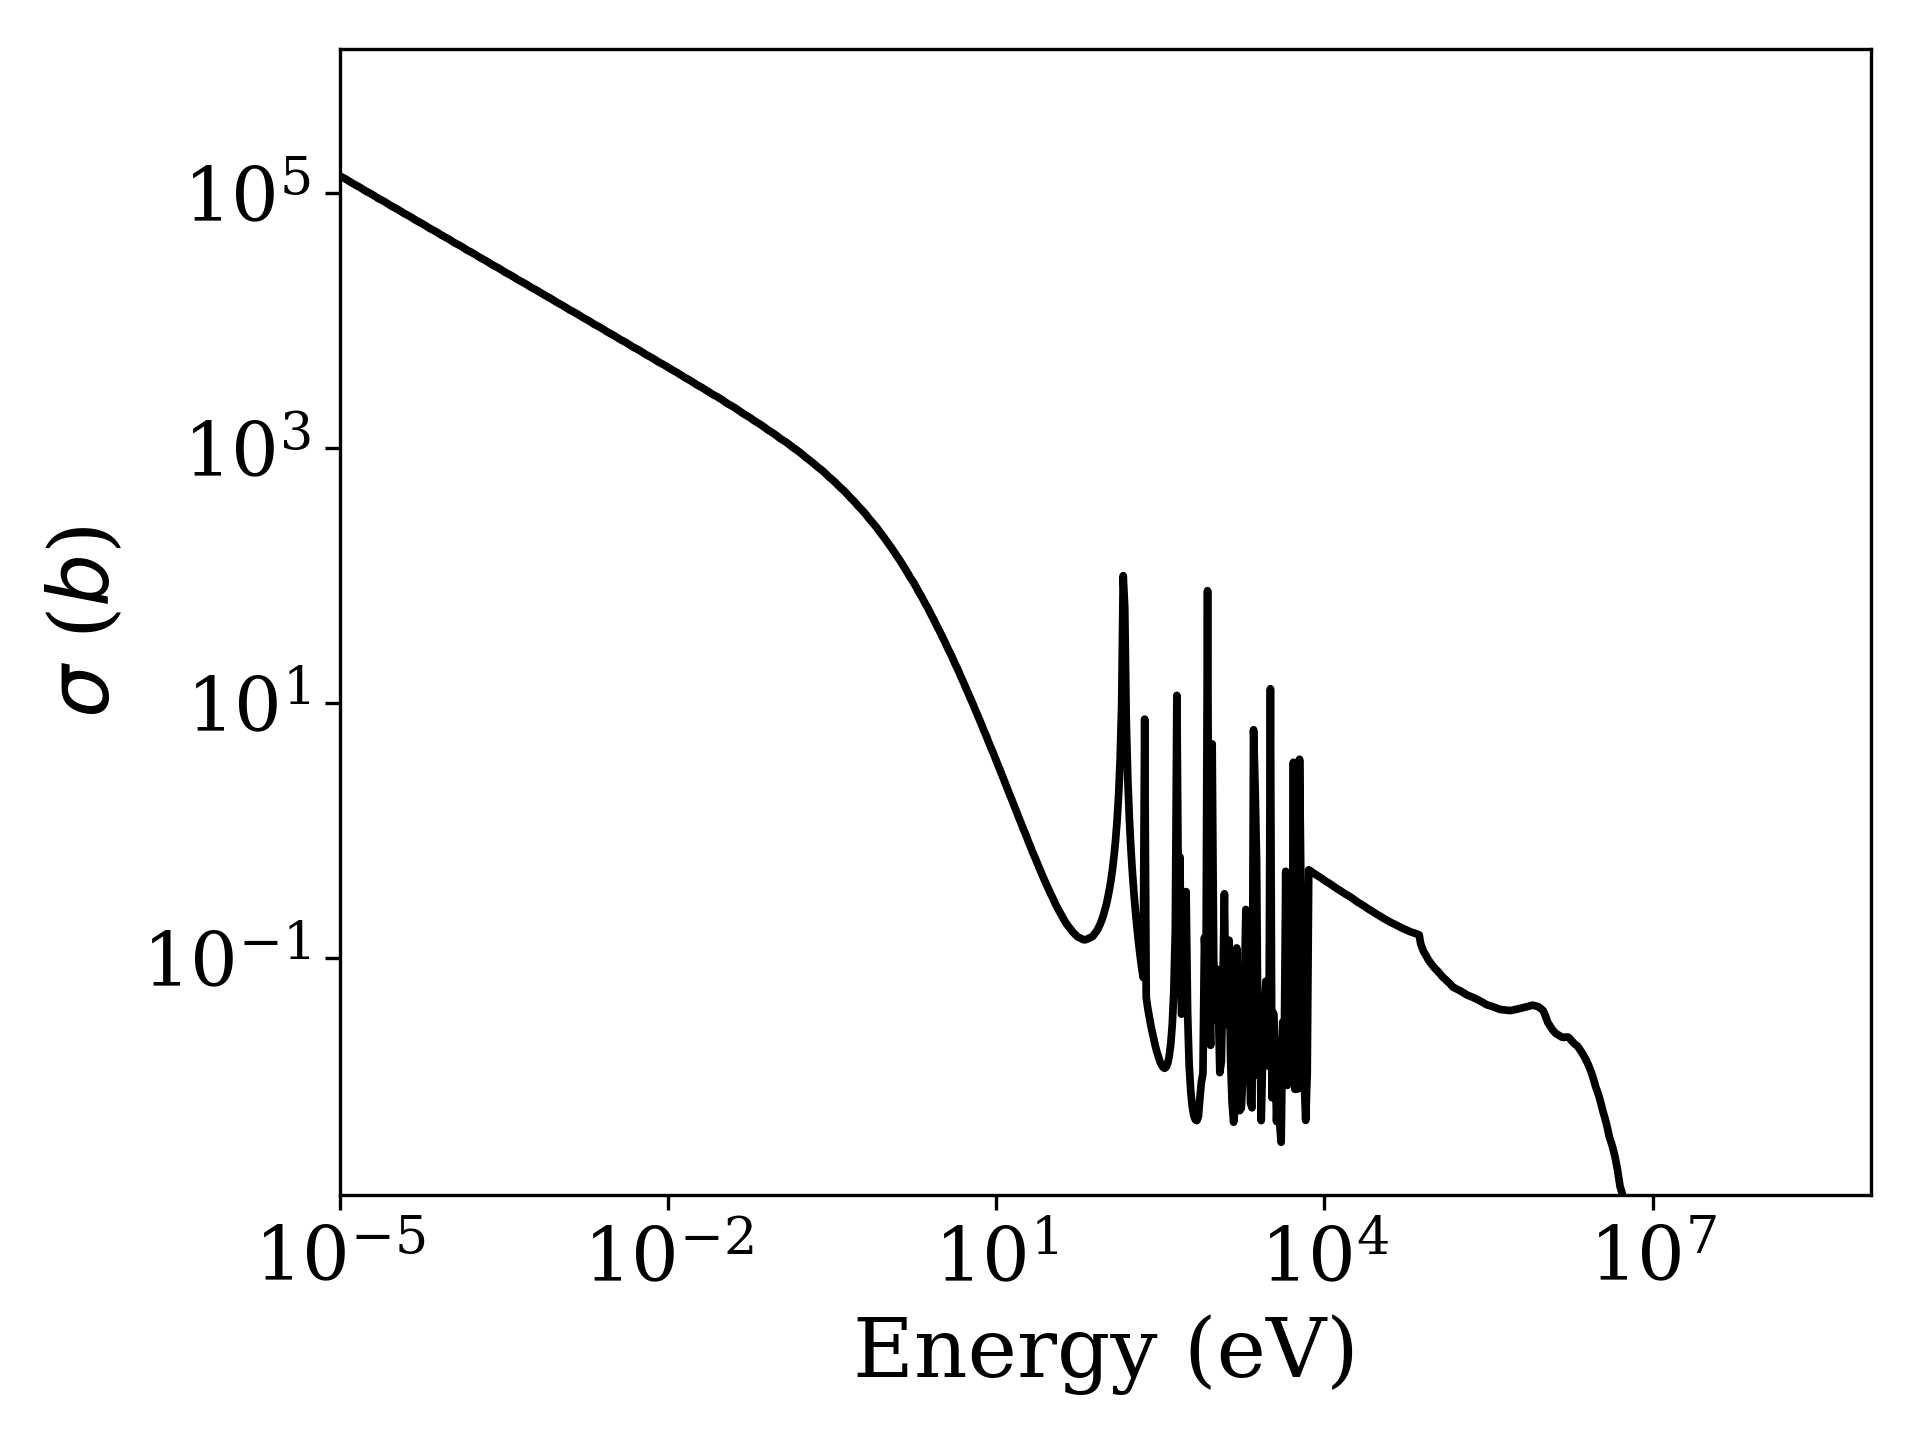
\includegraphics[width=.8\textwidth]{plot/Dy-164(n,gamma)Dy-165} 

  \caption{A subfigure}
  \label{fig:sub2}
\end{subfigure}
\caption{A figure with two subfigures}
\label{fig:test}
\end{figure}

\begin{table*}[h]
\centering
\begin{tabular}{ |c|c|c|c|c|c|c| }
 \hline
 Reaction & T$_{1/2}$ & ROI (eV) & Important Gammas (keV) \\
 \hline 
 $^{164}$Dy(n,$\gamma$)$^{165}$Dy &  2.4 h & 6.31e-03, 1.83e-01 & 108.16(0.0301) \\ 
\hline
\end{tabular}
\end{table*}
